%%
%% Author: jamie
%% 04/10/18
%%

% Document
\chapter{Empirical Studies}\label{ch:empirical}

\section{Overview}\label{sec:empOverview}
In this chapter we will cover a number of experiments that were conducted in order to investigate
the performance of the different algorithms implemented in order to tackle Leduc Hold'em.
We will begin with a simplified version of MCTS for POMDPs and will incrementally add to this
method in order to see how the performance of our agent evolves.
In the table below we have listed the template that we will follow when conduction these experiments.

\begin{tabular}{ | p{2cm} | p{10cm} | }
    \hline
    \textbf{Section} & \textbf{Rationale} \\
    \hline
    Objective & This section will contain an explanation of the purpose of the experiment along with
    how it was carried out \\
    \hline
    Algorithm and Coding & This section will go into the details of the algorithm used to produce results \\
    \hline
    Results & This section will detail the results acquired from the experiments conducted \\
    \hline
    Analysis & In this section we will examine our results and try to provide insight into the
    reasoning behind these results \\
    \hline
\end{tabular}

\section{Experiment 1 - UCT Versus Random Player}\label{sec:expmeriment1}
The first experiment conducted involved a simplified version of the algorithm outlined in\citep{silver2010monte}.
We set an initial goal of using a random player as our benchmark opponent in order to demonstrate how
this algorithm could exploit such a player's strategic inefficiencies.

\subsection{Objective}\label{subsec:objective1}
The goal of this experiment is to implement MCTS for Leduc Hold'em.
The MCTS agent will play against a random player and learn a strategy to exploit this player for
maximal reward.
Although we are interested in the results gained from playing against the random player we treat the
outcome of this experiment as a baseline for our subsequent results.
The reasoning for this is that the difficulty in finding a winning strategy against a random player
is not high.
Thus we expect that the exploitability of the resultant agent will be relatively high due to the
fact that it will not have learned all of the strategic intricacies of the game.
Rather, it will simply know how to beat a 'dumb' random player.
This will give us a platform to build a more sophisticated agent through different mechanisms such as
self-play in the subsequent experiments.

\subsection{Algorithm and Coding}\label{subsec:algAndCoding1}
As mentioned we will be following Silver's 2010 implementation.
The pseudocode for this algorithm can be seen below.
This algorithm ticks the box of being applicable to POMDPs like poker.
The one deviation from Silver's implementation is that we do not include the use of belief states.
Belief states are used in order to avoid the difficulty of learning a function with unbounded
input\citep{thrun2000monte}.
In our case we are learning values associated with histories of actions and observations that occur in the game.
Due to the nature of Leduc Hold'em these histories are limited in their length and thus belief states are
not required.

\begin{figure}[ht]
    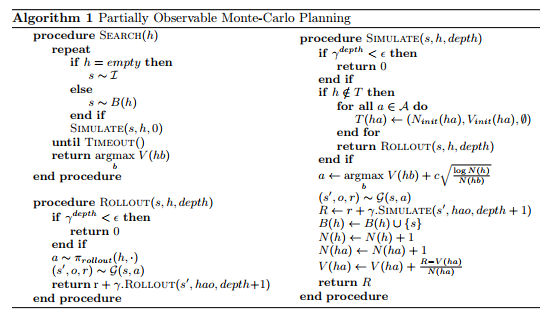
\includegraphics[scale=.8]{POMCTs_algorithm.png}
    \caption{Partially Observable Monte Carlo Planning}
\end{figure}

\lstset{language=Python}
\lstset{frame=lines}
\lstset{caption={Code will go here}}
\lstset{label={lst:code_direct}}
\lstset{basicstyle=\footnotesize}
\begin{lstlisting}
    import numpy as np
\end{lstlisting}

\subsection{Results}\label{subsec:results1}
The first metric that we used in order to analyse the results of this experiment is cumulative reward.
This is simply the sum of the output of the reward function over time.
In our case the function directly corresponds to the size of the pot won or lost in the game,
thus we can have either a positive or negative reward.
In figure 4.2 we see the reward over time increasing.
In order to obtain these results we ran the algorithm for 10000 iterations and repeated this process 100 times.
We then averaged our cumulative rewards at each iteration across these 100 repetitions to give the graph shown.
Figure 4.3 shows the rate of increase of cumulative reward.
In the case of figure 4.3 we applied the MCTS algorithm for 200000 iterations and
repeated this process 10 times, averaging the results.

\begin{figure}[ht]
    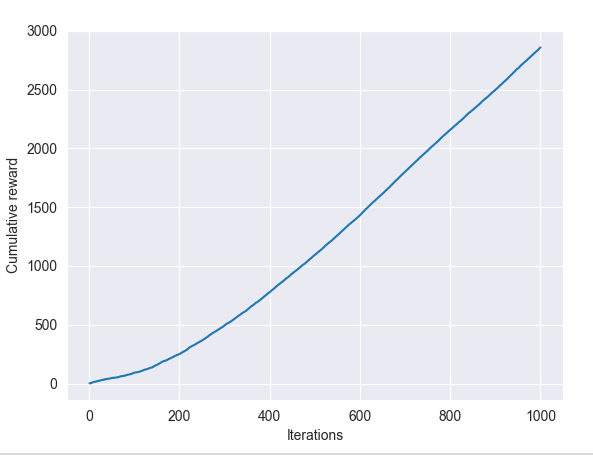
\includegraphics[scale=.8]{images/cumulative_reward_mcts_vs_random.png}
    \caption{MCTS cumulative reward over time vs random player - 10000 Iterations}
\end{figure}

\begin{figure}[ht]
    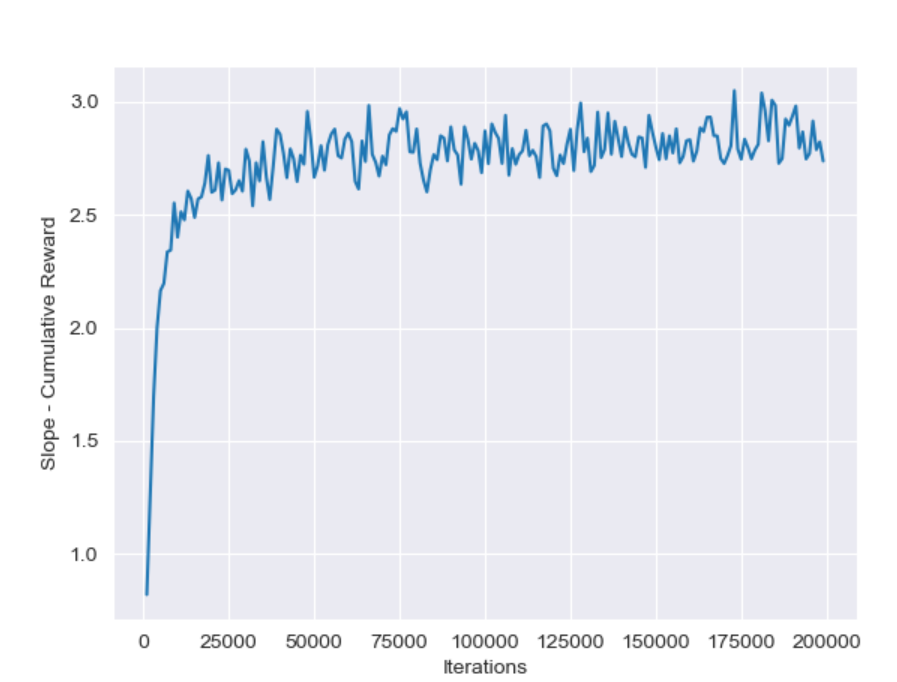
\includegraphics[scale=.8]{images/slope_cumulative_reward_vs_random_player.PNG}
    \caption{MCTS slope of cumulative reward over time vs random player - 200000 Iterations}
\end{figure}

The second metric used to produce results was exploitability.
This is a measure of the reward that can be gained by playing a best response strategy
against the agent.

\begin{figure}[ht]
    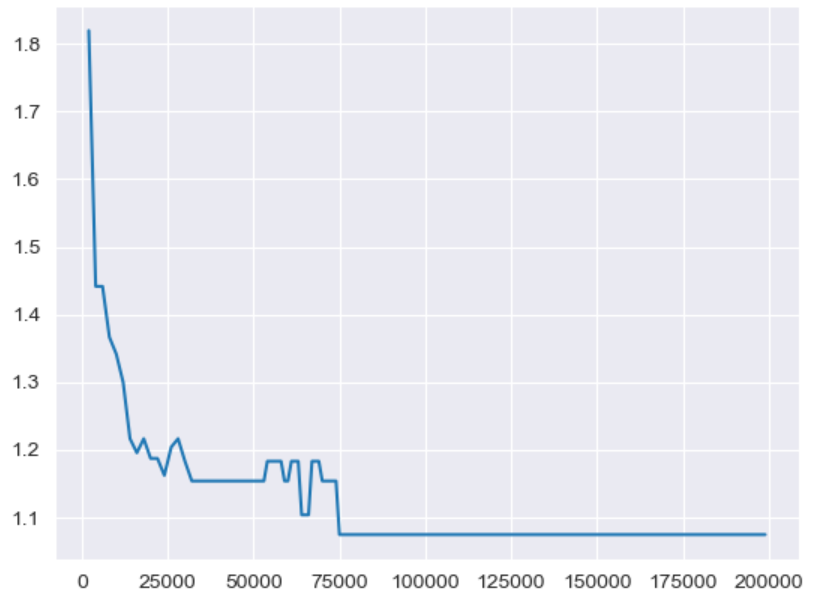
\includegraphics[scale=.8]{images/exploitability_vs_random_player.PNG}
    \caption{MCTS exploitability over time vs random player - 200000 Iterations}
\end{figure}

\subsection{Analysis}\label{subsec:analysis1}
We will first analyse our results from the cumulative reward metric.
As shown by figure 4.2 we see that initially there is a gradual increase in cumulative reward,
with the slope growing until there is a constant rate of increase.
This demonstrates that during the initial phase of the algorithm we have not yet uncovered
the most beneficial action selection for all states and the exploration phase is still in effect.
However, by visual inspection we can see that over time the rate of increase in cumulative
reward begins to stabilise which indicates that a concrete strategy that can exploit
the random play has been established.
This hypothesis is further supported by figure 4.3 as we see a dramatic upswing
in the rate of increase of cumulative reward followed by a levelling of the graph.

In figure 4.4 we see that the exploitabilty of the of the strategy generated begins
at roughly 1.8 and declines over time to less than 1.1 after 100,000 iterations.
This once again demonstrates that the agent is developing an intelligent strategy over time.
However the fact that we do not observe the exploitability value continue to converge towards
0 demonstrates that the strategy developed does not closely resemble a Nash's equilibrium
inducing strategy.
This is most likely explained by the fact that we are not playing against a rational player.
As such our strategy is strong when it comes to maximally exploiting an irrational, random player
but if we then substitute this irrational player for a rational player, the results will not be favourable.
\section{Experiment 2 - UCT Self-Play} \label{sec:experiment2}

\subsection{Objective}\label{subsec:objective2}
\subsection{Algorithm and Coding}\label{subsec:algAndCoding2}
\subsection{Results}\label{subsec:results2}
\subsection{Analysis}\label{subsec:analysis2}

\section{Experiment 3}\label{sec:experiment3}

\subsection{Objective}\label{subsec:objective3}
\subsection{Algorithm and Coding}\label{subsec:algAndCoding3}
\subsection{Results}\label{subsec:results3}
\subsection{Analysis}\label{subsec:analysis3}

\section{Experiment 4} \label{sec:experiment4}

\section{Experiment 5} \label{sec:experiment5}

\section{Experiment 6} \label{sec:experiment6}

\section{Experiment 7} \label{sec:experiment7}
